
\chapter{The Experiment}

\section{Large Hadron Collider}

The Large Hadron Collider (LHC) has a radius of approximately 27 kilometers. As of this writing, it is the largest machine ever constructed. The initial purpose of the LHC was to discover the Higgs boson, but it is capable of investigating a variety of other physics phenomena, such as dark matter, extra-dimensions, and heavy-ion physics.

The beams are accelerated along a circular path using radio frequency cavities, gaining energy with each revolution. LHC is a hadron collider, meaning it is designed to collide particles made of quarks and gluons. The proton-proton, proton-Pb, and Pb-Pb collision energies are the largest ever probed experimentally. The LHC is a circular collider.

Heavy-ion collisions at LHC produce strongly interacting nuclear matter. The temperature and density of this matter is comparable to the state of the universe only a few milliseconds after the Big Bang.

\section{Compact Muon Solenoid}

The Compact Muon Solenoid (CMS) is a general-purpose particle detector located at Point-5 of the LHC. CMS was designed to precisely measure the momentum of muons. The titular superconducting solenoid magnet was designed to generate a 4 Tesla field, but operates at 3.8 T to increase longevity. This field is homogeneous and parallel to the beam line close to the interaction point. The momentum of a muon is measured from how it deflects when moving through the magnetic field. Altogether, CMS weighs approximately 12,500 metric tons, with a diameter of 14.6 m and a length of 21.6 meters.

\begin{figure}[h!]
\begin{centering}
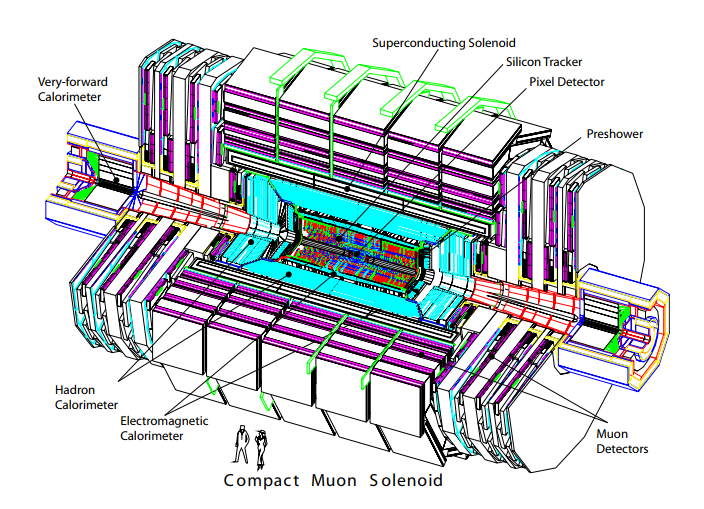
\includegraphics[width=4in]{Chapter3/importfigs/fromCMS_DesignPaper_perspective.png}
\par\end{centering}
\end{figure}

Within the solenoid volume are a silicon pixel and strip tracker, a lead tungsten crystal electromagnetic calorimeter (ECAL), and a brass and scintillator hadron calorimeter (HCAL), each composed of a barrel and two endcap sections. 


\begin{figure}[h!]
\begin{centering}
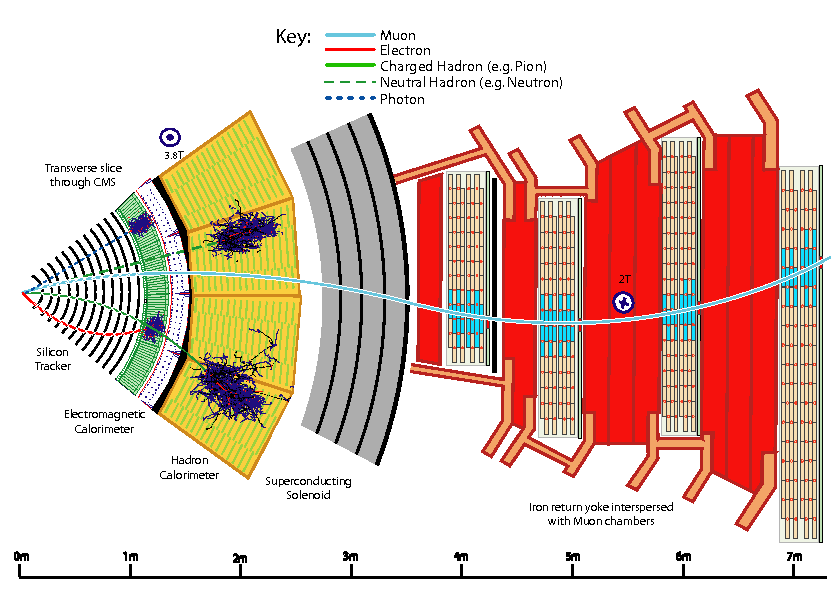
\includegraphics[width=5.5in]{Chapter3/importfigs/Figure_001.png}
\par\end{centering}
\end{figure}

\subsection{Tracker}

The tracker measures the momentum of charged particles via their trajectory through a homogenous magnetic field. The tracker consists of two units, the pixel tracker and the strip tracker, both of which are made of silicon. A charged particle causes an electrical signal when passing through a silicon pixel or silicon microstrip. CMS reconstructs these electrical signals, taken at specific points of position and time, into tracks. These tracks are accurate to 10 micrometers. The tracker is meant to have  a particle pass all the way through it, with only minimal effect particle's trajectory. 

The tracker system is designed for high granularity and fast readout, such that each trajectory can be associated with its corresponding bunch crossing. The tracker is resilient enough to withstand the high flux of particles accompanying every bunch crossing; at design luminosity of $10^34 cm^-2 s^-1$, some 1000 particles will traverse the tracker every 25 ns. However, the mass of the tracker is minimal enough to suppress multiple scattering, off its material, that would distort particle trajectories. These design constraints -- resistance and transparency -- are satisfied silicon. The tracker has approximately $200 m^2$ of silicon surface, making it the largest silicon detector ever constructed.

\subsubsection{Pixel Tracker}

Every silicon-pixel has a corresponding readout chip. The readout chips are soldered through the bump-bonding method. The readout chip amplifies signals from the pixel. The pixel tracker is precise enough to distinguish the vertices of tracks originating from short-lived particles, such as bottomonia. The innermost elements of the pixel tracker come within 4.4 cms of the CMS interaction point. The pixel tracker covers a pseudorapidity range of $|\eta|<2.5$ with some $66 \times 10^6$ separate pixels.

\subsubsection{Strip Tracker}

Outside the pixel tracker are the layers of the strip tracker. They function similar to the components of the pixel tracker, except the strip tracker consists of thin silicon plates. The strip tracker itself can be broken down into four components: the inner barrel layer, the inner endcaps, the outer barrel layer, and the outer endcaps. In total, these layers contain some $9.3 \times 10^6$ strips.

\begin{figure}[h!]
\begin{centering}
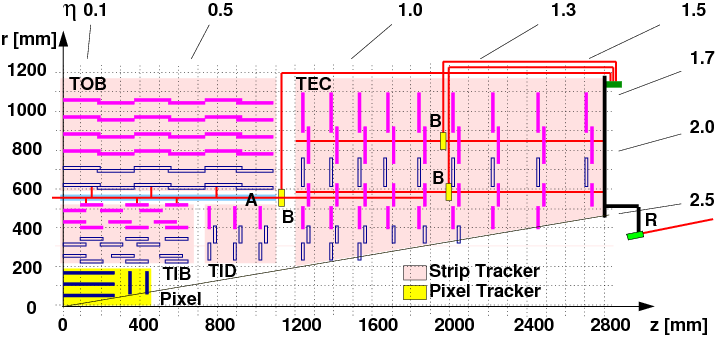
\includegraphics[width=4in]{Chapter3/importfigs/cms_cft_09_003_fig1.png}
\par\end{centering}
\end{figure}

\subsection{Electromagnetic Calorimeter}

The Electromagnetic Calorimeter (ECAL) is the dedicated CMS calorimeter for detecting electrons and photons. The calorimeter is comprised of lead tungstate ($PbWO_4$) crystals arranged in cylinder about the beam, including two endcaps. The granularity of these crystals gives the ECAL excellent energy resolution, angular resolution, and spatial resolution; for example, the ECAL has the resolution suitable for the decay of the Higgs boson into two photons. The ECAL is both hermetic and homogenous. 

\begin{figure}[h!]
\begin{centering}
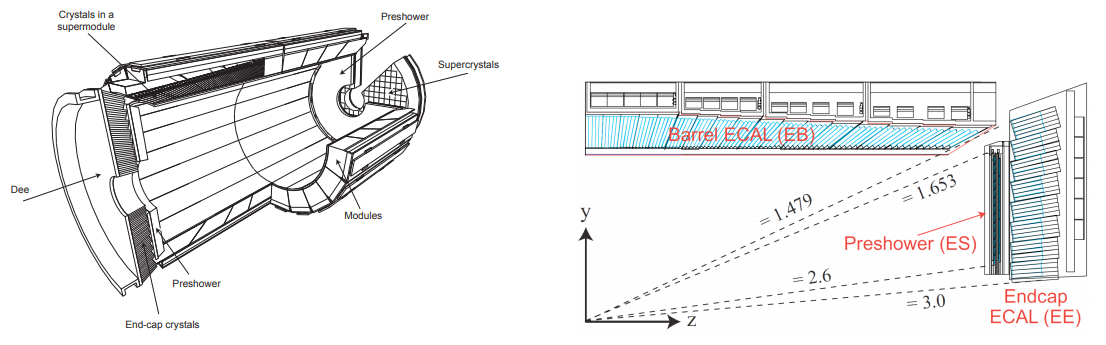
\includegraphics[width=7in]{Chapter3/importfigs/ecal_performance_with_examples.png}
\par\end{centering}
\end{figure}

The data readout is fast enough that CMS can trigger off signals in the ECAL. It takes about 25 ns for an ECAL hit to scintillate 80 percent of its lights, putting the calorimeter's rate on the same scale as the bunch crossing. Scintillation in the crystals activates photodetectors that transmit information to the L1 trigger. In the barrel these photodectors are avalanche photodiodes (APDs). The endcaps use vacuum phototriodes (VPTs).

\begin{figure}[h!]
\begin{centering}
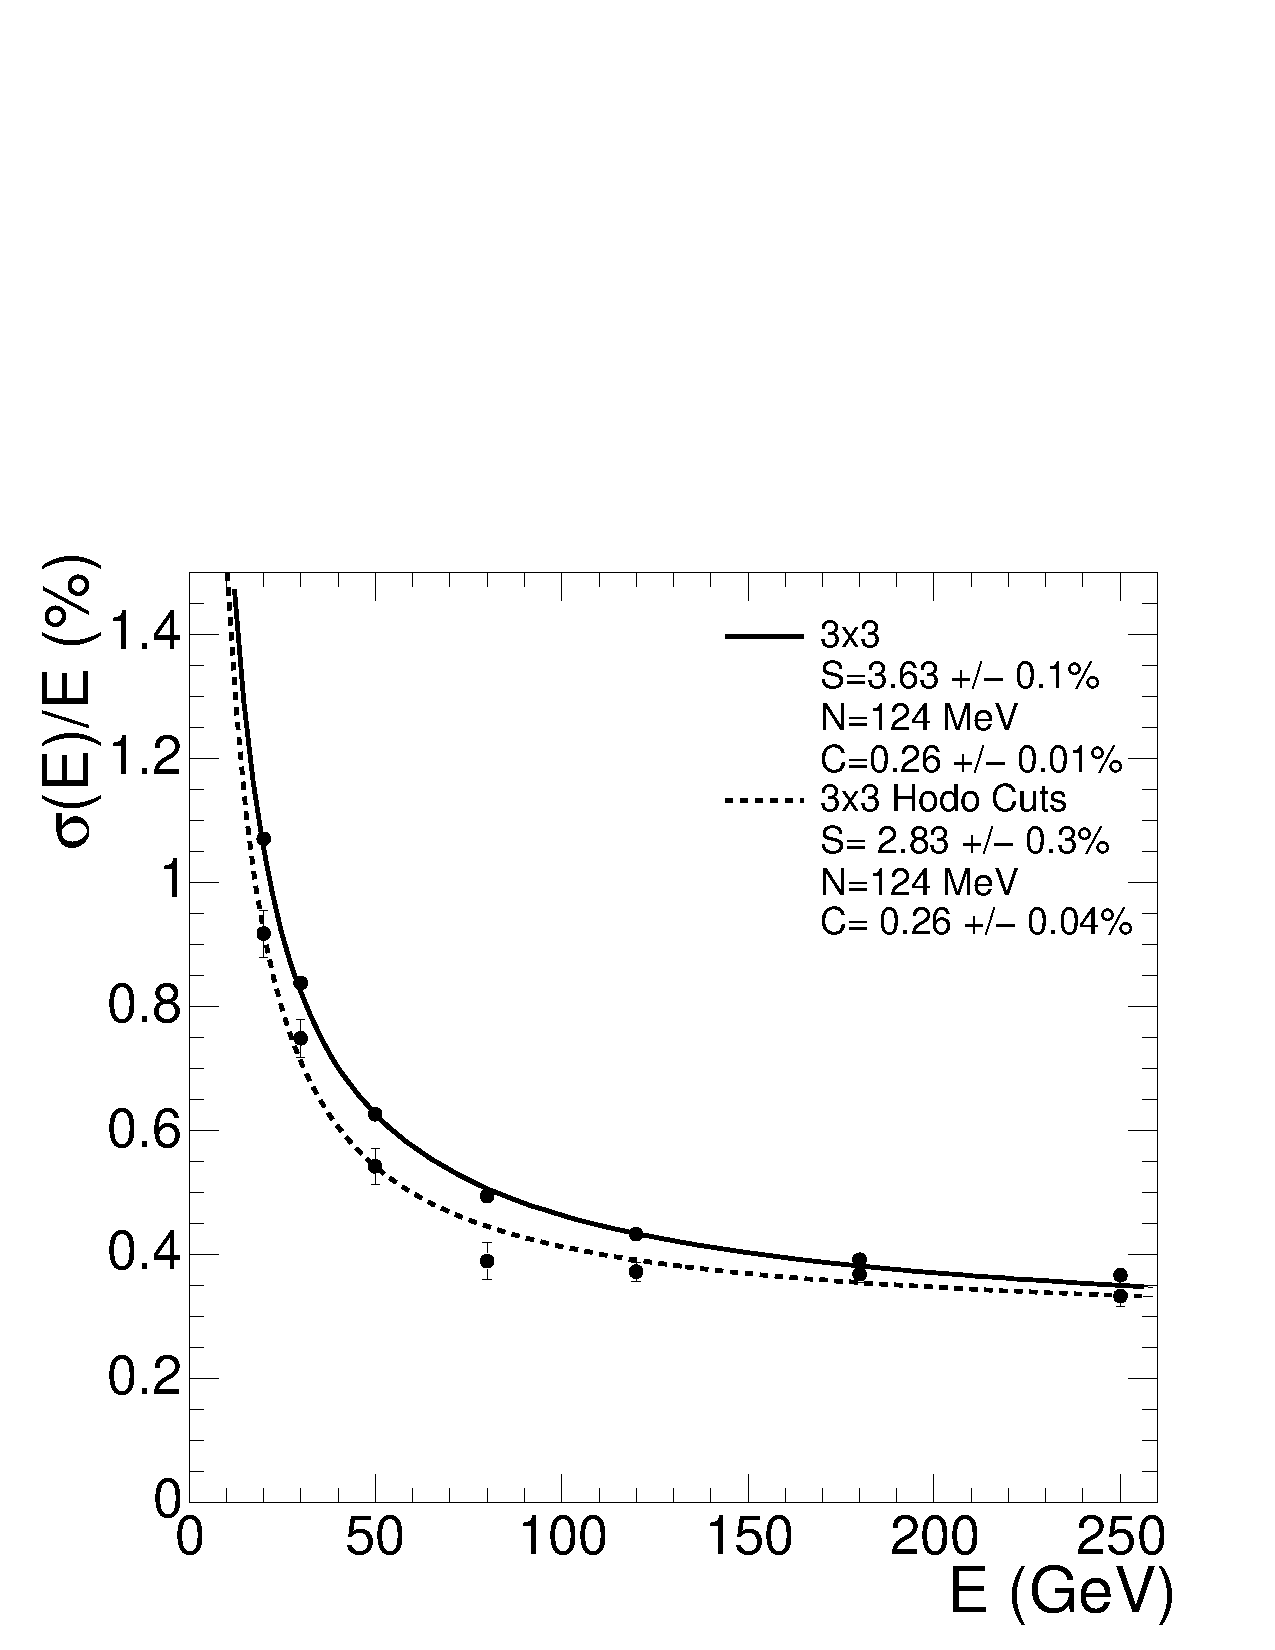
\includegraphics[width=4in]{Chapter3/importfigs/Figure_001-007.pdf}
\par\end{centering}
\end{figure}
 
\subsection{Hadronic Calorimeter}

\begin{figure}[h!]
\begin{centering}
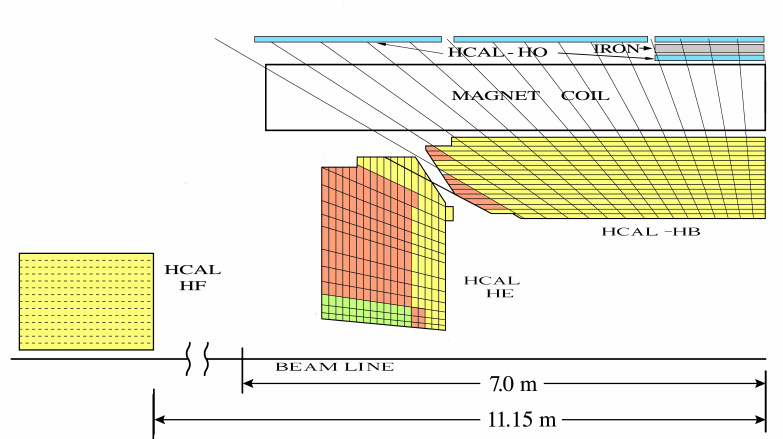
\includegraphics[width=5in]{Chapter3/importfigs/filtering_noise_in_CMS_hadron_calorimeter.png}
\par\end{centering}
\end{figure}

The Hadronic Calorimeter (HCAL) is the next layer outside the tracker. HCAL is a sampling calorimeter, meaning that it absorbs particles and measures their energyy and momentum via scintillation. HCAL has such a large acceptance that it can indirectly observe non-interacting particles such as neutrinos. The HCAL is designed to be hermetic, so that imbalances of momentum and energy can be precisely measured.


\begin{figure}[h!]
\begin{centering}
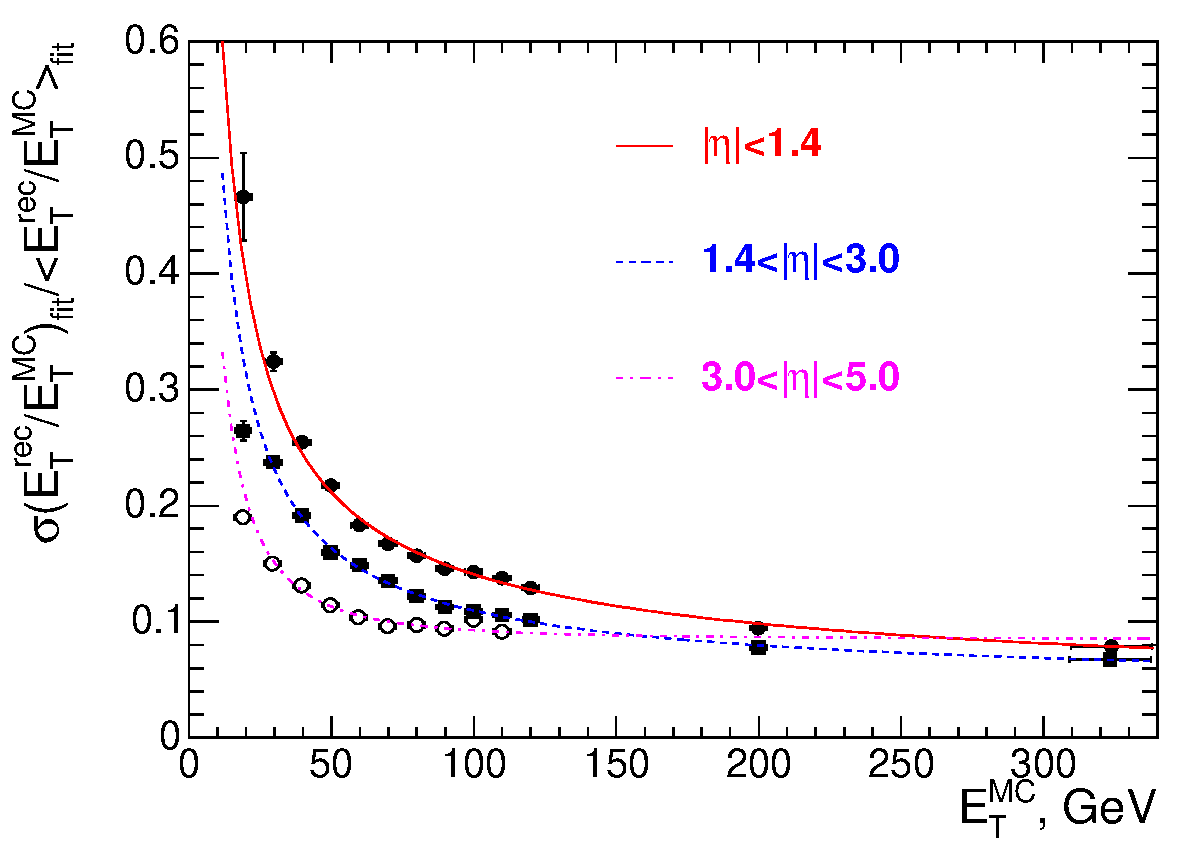
\includegraphics[width=4in]{Chapter3/importfigs/Figure_001-008.pdf}
\par\end{centering}
\end{figure}


\subsubsection{Hadronic Forward Calorimeters}

The Hadronic Forward Calorimeters (HF) absorbs the greatest portion of energy from collisions. As such it is designed for maximum radiative resistance. Hits in the HF are used to measure the instantaneous luminosity of CMS. The HF encompasses ($3.0<|\eta| < 5.2 $) and complements the coverage provided by the barrel and endcap detectors.

\subsection{Muon Detector}

The outermost layer of CMS consists of the muon detectors. Muons are particles nearly identical to electrons, except for their mass, which exceeds that of the electron by some two orders of magnitude. High mass particles, like the Higgs boson, often decay into a final state containing muons. The muon detector not only identifies muons, but also measures their momentum. The muon detector has readout fast enough for triggering on muons.

\begin{figure}[h!]
\begin{centering}
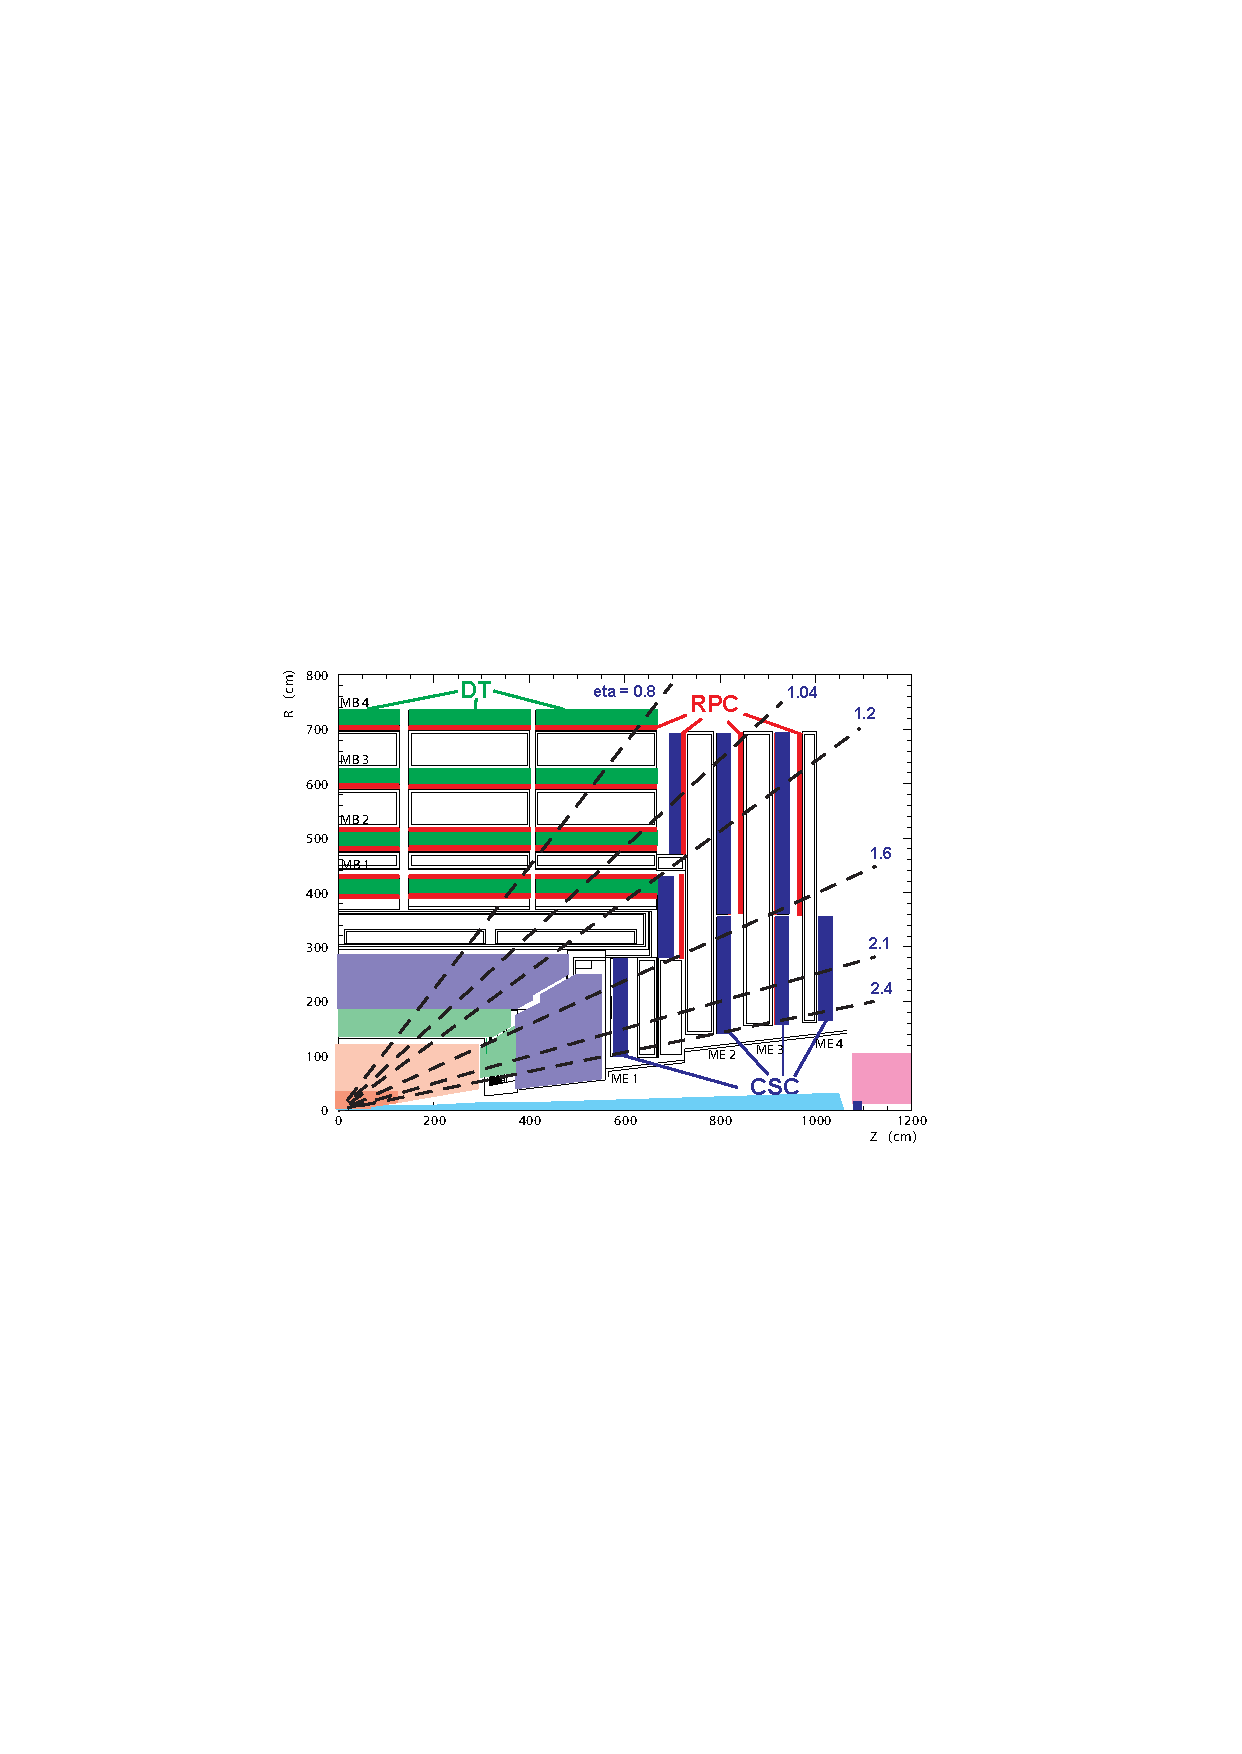
\includegraphics[width=4in]{Chapter3/importfigs/Figure_001-006.pdf}
\par\end{centering}
\end{figure}


\subsection{Zero Degree Calorimeter}

The zero degree calorimeters are both sides of CMS, approximately 140 meters from the interaction point. Each ZDC consists of two independent systems: an electromagnetic calorimeter, for detecting very forward photons, and a hadronic calorimeter, for detecting neutrons. Because these neutrons result from the dissociation of nuclei, the ZDC can measure the centrality of heavy-ion collisions. Hadrons in the forward region have energy on the TeV scale, so the ZDC's hadronic calorimeter is made of thick tungsten plates. For a UPC process, the photon emitting nucleus is most likely to remain intact; therefore, ZDC data can the photon direction of a process, and by extension it's energy. 

\subsection{Particle Flow Algorithm}

Raw data from the sub-detectors is combined, for data analysis, by the particle-flow (PF) algorithm. The PF takes the data about tracks in the tracker and energy deposits in the calorimeter, and uses them to reconstruct physics-related data objects, like jets, and to identify specific particles, such as photons and muons. The PF also identifies missing energy and momentum for use in neutrino studies. These data objects are stored in a format similar to that of conventional MC event generators. CMS gains significant jet reconstruction efficiency via the PF. At low transverse momentum, PF reconstructs jets at nearly twice the resolution of HCAL and ECAL. This increase in efficiency comes from the PF integrating in track data with the calorimeter tower data. 

\begin{figure}[h!]
\begin{centering}
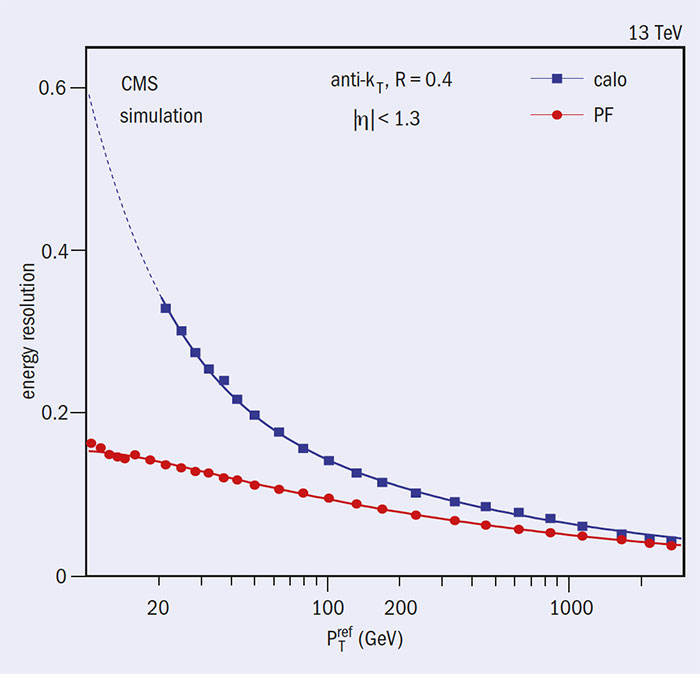
\includegraphics[width=4in]{Chapter3/importfigs/CCrec2_05_16.jpg}
\par\end{centering}
\end{figure}

\subsection{Luminosity}

One of the most important quantities measured by CMS is luminosity. Luminosity is necessary to convert the number of events detected, for a given channel, into a collision cross-section. Collision cross-sections are among the primary observables predicted by theoretical physics, specifically quantum field theory. For particle physics, the collision cross-section of a process is typically measured through the relation:

\begin{equation}
\sigma  = \frac{R}{\mathit{L}}
\end{equation}

Where $\sigma$ is the cross-section, $R$ is the rate at which the process occurs per collision, and $L$ is the luminosity.

\subsubsection{van de Meer Scanning}

The luminometers of CMS produce signals proportional to the instantanteous luminosity of the LHC beam. However, these signals need to be properly calibrated with respect to a known visible cross-section for each luminometer. This calibration is accomplished via Van de Meer scanning. The opposing beams of LHC are moved back and forth in the transverse plane. During the scan, the detector response is measured as a function of beam displacement. The beam widths are calculated from Gaussian fits to the detector response. The visible cross-section of the luminometer in question is then derived from the width of the beams, and acts as the calibration of the detector response. 

\subsection{Triggering}

CMS uses a two-tiered triggering system. The first tier, the L1 trigger, is hardware based. The second tier, the high-level trigger (HLT), is software based. The L1 trigger recieves raw data from the calorimeters and the muon detectors; this determines when the tracker will readout data. The raw data from the tracker, calorimeters, and muon detectors is then passed on to a computer farm running the HLT menu. The HLT then performs a simplistic reconstruction of the raw data into physics objects useful for analysis: jets, tracks, and identifiable particles. If an event passes the HLT, the raw data is permanently stored in preparation for a more complex reconstruction. 

The 2015 UPC triggers were for low multiplicity events and low transverse momentum events. Typical heavy-ion collisions are high multiplicity events. Below is an event from one of the first heavy-ion collisions at CMS in 2010.

\begin{figure}[h!]
\begin{centering}
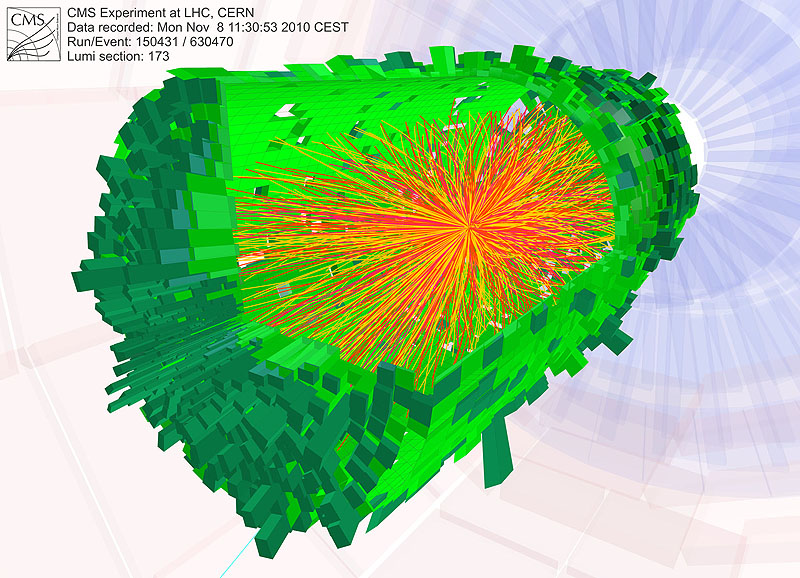
\includegraphics[width=4in]{Chapter3/importfigs/cms_firstleadcoll.jpg}
\par\end{centering}
\end{figure}

The event below is an example of a UPC upsilon candidate.

\begin{figure}[h!]
\begin{centering}
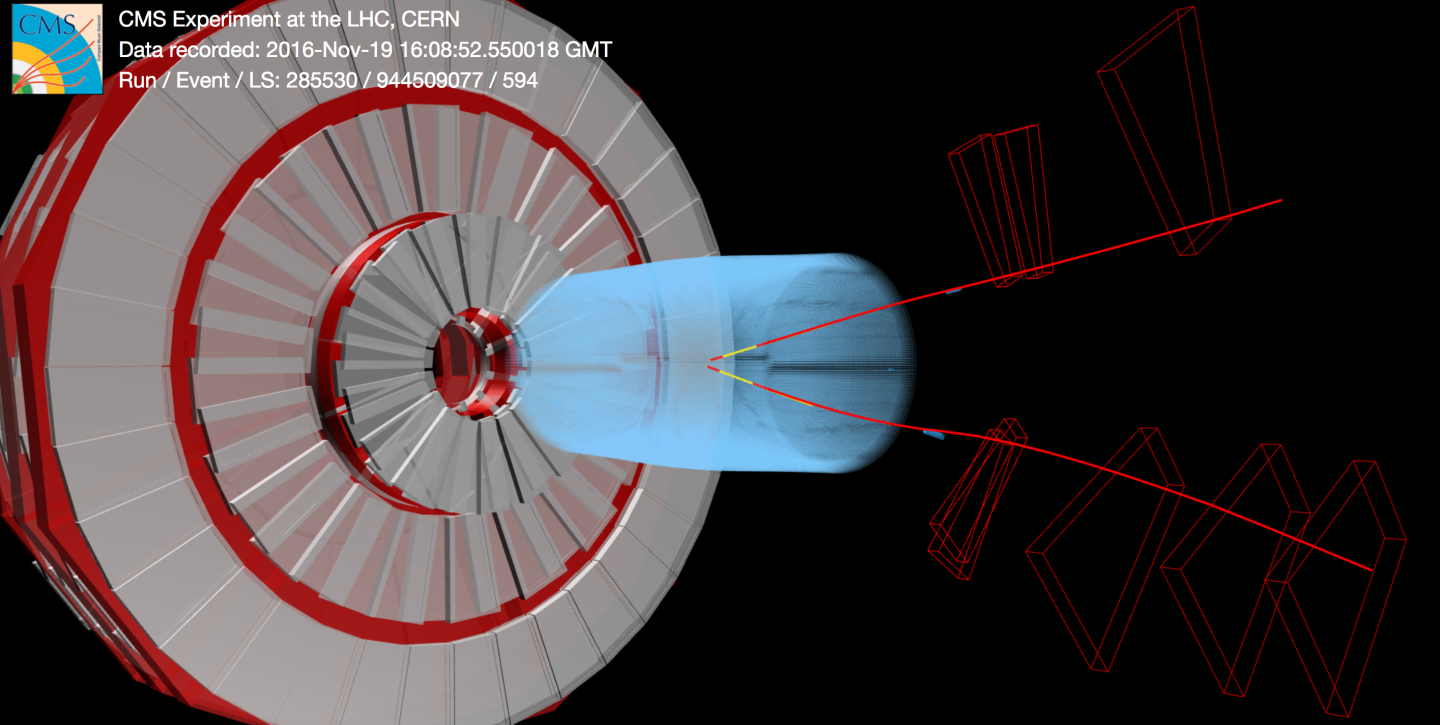
\includegraphics[width=4in]{Chapter3/importfigs/upcJpsi_run285530_lumi594_event944509077_v0.png}
\par\end{centering}
\end{figure}

For this analysis, the L1 trigger applies two selections. First, the L1 checks that at least one of the HF is empty. This is the most important part of the trigger in so far as it suppressed the hadronic contamination of the dataset. Then, if there is at least 5 GeV of energy deposited in the ECAL, the event passes to the HLT. 

Low multiplicity events are difficult to distinguish from background. To compensate, the HLT in turn requires that there be at least once reconstructed track from the pixel tracker, to make sure that there are particles that will be reconstructed by the complete tracker. Only the pixel tracker is used for these HLTs to increase the speed of reconstruction while decreasing needed computer cycles. 